\chapter{An Approach to Semantic Discovery}

The backbone of the Web of Things is Semantic Web technology and its clever reuse of established standards to ease the M2M communication, instead of creating novel recommendations. So it makes sense, that the goal of this work is to prove the feasibility of query-based discovery algorithms using only RDF and SPARQL. 

Recall Tricia, who wanted to avoid building a complex vertically integrated system on her own. Now assume she has read a bit about the WoT and would like to apply this to her system. She has TDs for all of the devices, she would like to monitor. That was the easy part, now she has to configure the network and find out which devices should be communicating with one another. The algorithms presented in this chapter will help her achieve this goal with minimal interaction. She understands that the basis of the WoT is to recycle recommendations and to keep her programming as abstract as possible, so she uses the RDF framework and SPARQL to exchange this data.

Both discovery algorithms are based on the consideration that related semantic graphs are necessarily redundant. The proposed discovery algorithms leverage this simple concept by identifying redundant blank nodes in each RDF graph. For example: if NodeMCU 1, which is mapped to the water level sensor wants to affect the water level, it must interact with NodeMCU 3, which controls the valve leading to the same tank.

A third algorithm, which is only used in the centralized discovery algorithm, was implemented. This algorithm runs on a PC client and computes the graph redundancies from two microcontrollers and then sends the leaned RDF graphs back to the microcontrollers.

\section{Graph Theory Refresher}
This work requires some working knowledge of graph theory. There are a few definitions that will be helpful before continuing, including some definitions that are specific to RDF. Listed below are helpful definitions.

\begin{itemize}
    \item A (directed) graph is \textbf{strongly connected} if each node is reachable by following a directed path. If the graph is connected by ignoring path direction, than that graph is \textbf{weakly connected}.
    \item A graph, $G'$ is considered to be a \textbf{proper subgraph} of $G$ if, the group of vertices in the subgraph, $V'$, is a proper subset of $V$ or the edges $E'$ are a proper subset of $E$. Proper in this case means the subset is not equal to the original set. Applied to RDF, a proper subgraph is a proper subset of the triples in an RDF graph.
    \item An \textbf{instance} of an RDF graph is created by replacing some (or all) of it's blank nodes to some set of literals, IRIs, or other blank nodes. Any graph is an instance of itself. Instances are a transitive relation, meaning an instance of an instance of a graph $G$ is also an instance of $G$. \cite{RDFSemantics.Hayes.2014}
    \item An RDF graph is considered \textbf{lean} if there is no instance in a graph, which is a proper subgraph of itself. A non-lean graph contains internal redundancies and expresses the same semantics as their lean subgraph. \cite{RDFSemantics.Hayes.2014}
    \item Two graphs are \textbf{isometric} if, they can be mapped to each other by a 1:1 mapping on their blank nodes. Isometric graphs are treated as being more or less identical, since blank nodes have no identity other than their location in the graph. \cite{RDFSemantics.Hayes.2014}
    \item A \textbf{Connected Subgraph} of a graph $G$ is a subgraph of $G$ containing at least one blank node (as a subject or an object). If a graph contains more than one blank node, then the blank nodes make up a chain, meaning it is possible to navigate through to the next blank nodes by following a directed path until a non-blank node\cite{Esposito.2005}. As an example consider the LUT400 data from figure \ref{fig:rdflut400}, the data starting at \texttt{urn:tank} to the CoAP web resource forms a blank node connected graph; this connected subgraph contains two blank nodes, \texttt{b1} and \texttt{b2}.
\end{itemize}

Here's an example from the W3C\cite{RDFSemantics.Hayes.2014} of an non-lean graph, represented in triples: \newline
\begin{center}
\texttt{ex:a  ex:p  \_:x .} \newline
\texttt{\_:y  ex:p  \_:x .} \newline
\end{center}

Why is this example not lean? If the blank node \texttt{\_:y} were mapped to \texttt{ex:a}, then the triple in the second line would be equal to the first triple. Meaning the instance is a proper subgraph of itself, and therefore is not lean. Now consider following example, also from the W3C\cite{RDFSemantics.Hayes.2014}. Is this graph lean? \newline

\begin{center}
\texttt{ex:a  ex:p  \_:x .} \newline
\texttt{\_:x  ex:p  \_:x .} \newline
\end{center}

Yes, it is lean! There is no mapping for \texttt{\_:x}, which can make the second triple equivalent to the first. Recall, that the reflexive relationship is not allowed, so \texttt{ex:a  ex:p  ex:a .} is not valid, thus \texttt{\_:x} can't be mapped to \texttt{ex:a}.

\section{Implementations}
This section presents three algorithms that were implemented during this case study. The first algorithm culls redundant blank nodes and builds \textit{lean} semantic graphs for the centralized discovery algorithm. The second algorithm discussed will be the centralized discovery algorithm. The final algorithm that will be presented is the decentralized discovery algorithm.


\section{Reducing Redundancies in RDF Graphs}
\label{graphlean}
The previous chapter discussed the W3C RDF recommendation. RDF graphs are a simple way for machines to represent semantic data, but their complexity and size grows explosively as information increases. Therefore, several researchers have put great efforts into reducing the number of blank nodes in an attempt to reduce query times\cite{Esposito.2005}. This is equivalent to computing the \textit{lean} subgraph of the union of all RDF graphs on the network. From the definition of a lean subgraph, it's implied that each non-lean graph has an equivalent and unique lean subgraph\cite{Cyganiak.2014}. In her 2005 paper \textit{REDD: An Algorithm for Redundancy Detection in RDF Models} Floriana Esposito (et al.) \cite{Esposito.2005} created an algorithm with the intention of reducing query times by using this observation to compute lean graphs. Her intention was to reduce query times from graphs that had a large number of blank nodes.



Although the FESTO demonstrator only has five devices attached to it, which are controlled by only three microcontrollers, its combined graph is quite large--the leaned union graph contains twenty blank nodes, whereas the non-lean union contains thirty blank nodes. Figure \ref{fig:festoUnion} shows the core graph of the FESTO demonstrator. The blue nodes are blank nodes and the red nodes are redundant blank nodes. The leaned sum of all of the semantic graphs in the network will be referred to as the \textit{core} of the network. Looking at that significant reduction, it is easy to see the motivation for the REDD algorithm, in fact according to a 2014 survey on blank nodes, about 7.5\% RDF data across all domains were blank nodes\cite{Mallea.2011}.

\begin{sidewaysfigure}
	\centering
	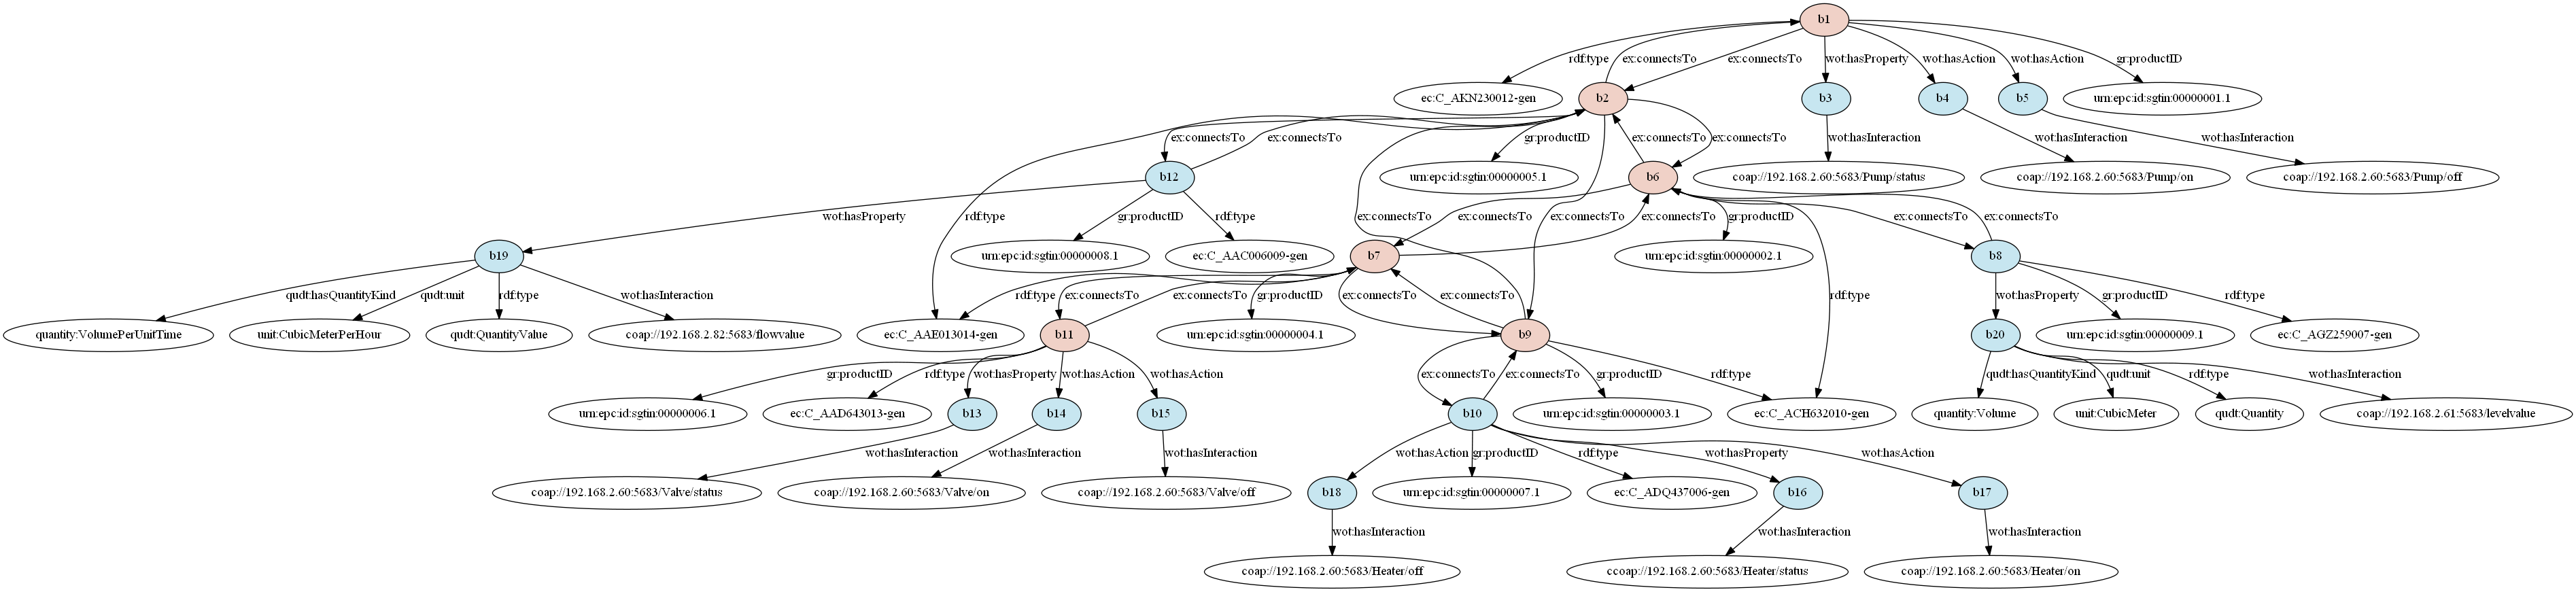
\includegraphics[width=\textwidth]{Figures/RDFUnion.png}
    \caption{Core RDF Graph from the FESTO Demonstrator; the leaned union of all the semantic graphs.}
    \label{fig:festoUnion}
\end{sidewaysfigure}

To do this she started by finding the connected subgraphs within each RDF graph, then taking the created connected graph and converting it to a query, then executing this query against another connected graph from a different set of semantic data. The resultant binding from this query should then be saved in a list and the set of bindings saved as the graph redundancies. Unfortunately, this did not actually reduce query times as much as desired, especially since running the algorithm took so long, but the algorithm presented by Esposito can be leveraged to create the centralized discovery algorithm.

The REDD algorithm proposed by Esposito has three steps: \change{this may be a bit unclear...}
\begin{enumerate}

\item  Build connected graphs from a given RDF graph, $m$
\item Convert each resultant connected graph into a query.
\item  Execute each query against the original graph, $m$.
\item  The set of results are the redundancies in the graph.

\end{enumerate}
Looking closer at the pseudocode in figure \ref{fig:EspositoListing}, we can see she starts by creating a set of connected graphs from one RDF graph in the function declared \texttt{Set CreateConnGraphs(Model m)}. Please note, that she using many of the naming conventions from the Apache Jena library, this library will be discussed in more detail, when we discuss the implementations of these algorithms. Suffice it to say: a model is a just another word for an RDF graph, and a statement is another word for an RDF triple. This means a model is composed of multiple statements, each of which has a subject, predicate, and object.

\texttt{CreateConnGraphs} starts by initializing an empty set for the connected graphs and a map to map the blank nodes to their respective connected graphs. The statements in model \texttt{m} are iterated over. If the statement contains a blank subject then it's checked if that particular "connected" graph is already mapped to that same blank subject, if so the statement is added to the current connected graph. If not a new blank graph is created for the statement and a that new graph is added to the set of connected graphs and the mapping of the blank subject to the connected graph is added to the map \texttt{blanksTocg}. An analogous process occurs for blank objects. \change{should you compare and contrast here?}

\begin{figure}
	\centering
	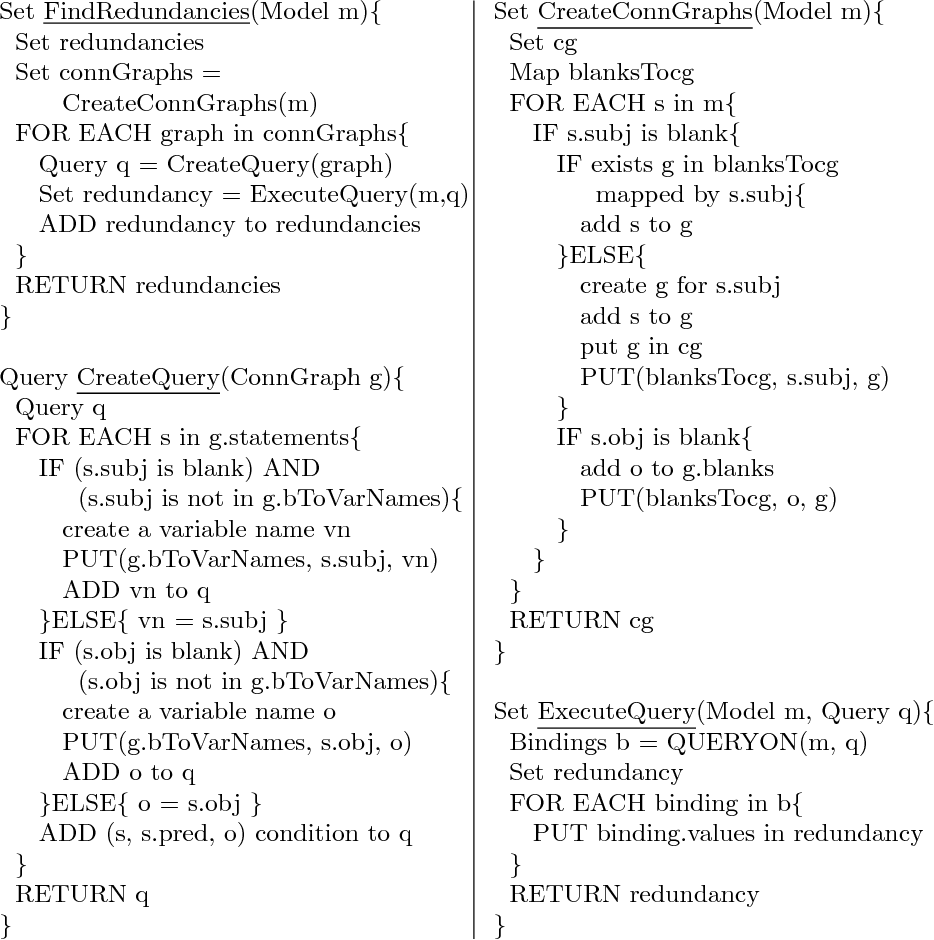
\includegraphics[width=\textwidth]{Figures/REDDlisting.png}
    \caption{The REDD Algorithm as presented in Esposito's 2005 paper.}
    \label{fig:EspositoListing}
\end{figure}

After the connected subgraphs are determined, the algorithm builds queries from the connected graphs in the function \texttt{CreateQuery}. Working through each triple in the connected graph, the query is generated by replacing any blank nodes with query variables. The variable names are come from a map, which as you can see is undefined and unclear, how these were determined. Unfortunately in Apache Jena this is quite a problem and is something that was worked around.

In the third step the queries are executed against the same original model and the query result is added to the set for the redundancies. Executing all of the queries against the original model yields all of the redundancies in the graph. Meaning we find if the original graph can be represented by one of its subgraphs.


The implementation in this thesis followed a similar approach to Esposito. First the algorithm computed the connected graphs in a given RDF graph. These connected graphs are also saved in a set and the blank node mappings to the connected graphs are noted. The connected graphs are then converted to queries, this does not require an extra function as in the Esposito implementation, since a Model can be converted to a query in Apache Jena, then the connected graph queries from the first model are computed against the second model. The same process is then done for the second model to be queried against the first. The algorithm returns a set of RDF node pairs, which are the redundant nodes that will be used by the centralized discovery algorithm.





\lstinputlisting[label={lis:reddPseudo}, caption={The pseudocode implemented in this thesis}, tabsize=2, breaklines=true, frame=single]{Code/reddPseudo.txt}
\vspace{1cm}

Finally, the structure of the algorithm was mostly retained, but extended to summarize two RDF graphs contents. How the REDD algorithm was integrated in the centralized discovery algorithm will be discussed in the next section. The details of the REDD algorithm's implementation will be discussed in the next chapter.



\section{Centralized Discovery}
The centralized discovery was used as a baseline. It works by gathering all of the in-network servients' data and executing the \texttt{GraphLean} algorithm locally. The pairs of redundant nodes returned by \texttt{GraphLean} are then used to update each servient's graph, which works as the algorithm below outlines.

The original RDF graph is $G_{i}$, which must be updated in the discovery algorithm. For this two graphs are created: $G^{-}_{i}, G^{+}_{i}$. $G^{-}_{i}$ stores triples that contain redundant blank nodes, which is subtracted from the original graph in order to create $G^{+}_{i}$. Mathematically: $G^{+}_{i} = G^{i}/G^{-}_{i}$. The centralized discovery works in twos, meaning pairs of semantic graphs are combined. This the number of pairs that are built would be ${n \choose 2}$, where $n$ is the number of semantic graphs in the network. So that means the REDD algorithm must be run at least ${n \choose 2}$ times, since it must run once for each unique pair.

A more precise expression of this update is below:

%For every original RDF graph, $G_{i}$ which should be updated two graphs are created:  The former is used for the redundant blank nodes, the later is the updated graph generated by adding all statements in the difference of . \change{this explanation may be hard to understand}

%This code has been commented out, it is deprecated
\begin{comment}
\change{this has gotten longer, pls change}
\begin{algorithm}
  \caption{Centralized Discovery}\label{centralized}
  \begin{algorithmic}[1]
    \Procedure{Update Servient Graphs}{$G_{1},G_{2}$}\Comment{Update Graph}
    \ForAll{($X_{1}, X_{2}$)} \Comment{$X_{i} \in G_{i}$}
    	\If{$\exists$ Triple $t$ : $t = (X_{1}, $\texttt{wot:hasInterationPattern}, $prop) \in G_{1}$}
      \State $t'\gets (X_{2}, $\texttt{wot:hasInterationPattern}, $prop)$
      \State Add $t'$ to $G_{2}$
      \ForAll{$t$ such that $t = (prop, p, o) \in G_{1}$} \Comment{$o$ is not blank}
      	\State Add $t$ to $G_{2}$
      \EndFor
      \EndIf
    \EndFor \Comment{Repeat with $X_{1}$ and $X_{2}$ swapped}
    \EndProcedure
  \end{algorithmic}
\end{algorithm}
\end{comment}

\begin{enumerate}
    \item Let $G_1, G_2, G^+_1, G^+_2, G^-_1, G^-_2$ be RDF Graphs
    \item For all pairs of RDF nodes ($X_1, X_2$), where $X_1 \in G_1$ and $X_2 \in G_2$,
    \begin{enumerate}
    \item \begin{enumerate}
        \item for all $t \in G_1$ with the form $(X_1, P, O)$,    add $(X_2, P, O)$ to $G^+_2$ and add $t$ to $G^-_1$
        \item for all $t \in G_1$ with the form $(S, P, X_1)$,    add $(S, P, X_2)$ to $G^+_2$ and add $t$ to $G^-_1$
    \end{enumerate} \item \begin{enumerate}
        \item for all $t \in G_2$ with the form $(X_2, P, O)$,    add $(X_1, P, O)$ to $G^+_1$ and add $t$ to $G^-_2$
        \item for all $t \in G_2$ with the form $(S, P, X_2)$,    add $(S, P, X_1)$ to $G^+_1$ and add $t$ to $G^-_2$
    \end{enumerate}

    \end{enumerate}
    
    \item For all $t \in G_1/G^{-}_1$, add $t$ to $G^{+}_{1}$
    \item For all $t \in G_2/G^{-}_2$, add $t$ to $G^{+}_{2}$
\end{enumerate}

The RDF Node pairs, $(X_1, X_2)$ in step 2 are determined by our version of the REDD algorithm. In 2.a the triples from $G_1$ containing the redundant blank node $X_1$ is added to the graph $G^-_1$, the triple containing the other node in this pair is added to the graph $G^+_2$. This occurs in 2.a.i for the redundant blank node as a subject, and in 2.a.ii for the node as an object. 2.b is analogous, but processes triples containing $X_2$. The third and fourth steps add the remainder of the triples that do not contain any redundant blank nodes to their respective graphs. The updated Graphs $G^{+}_{1}$ and $G^{+}_{2}$ are then sent to the servients.

To cut down on the total time of the algorithm and reduce unnecessary message passing, we chose to load all semantic data at the beginning of the benchmark onto the PC and run the update for the algorithm several times and then send the updated graphs back to the NodeMCUs.

\section{Decentralized Discovery}
The decentralized algorithm is very simple: each device broadcasts one or more queries to the network to which only devices with a non-empty answer should respond. This can be accomplished with just a few lines of code; the broadcasting requires only one line. Though the downfall of this is that there is significantly more overhead, since each servient broadcasts their connected blank node graphs.

For each connected blank node graph $G_i^{b}$ in the RDF graph $G_1$, $G_1^{b}$ should be constructed into a query by replacing the blank nodes in $G^{b}_{1}$ with query variables. This query is then broadcasted to the network. Each device broadcasts as many queries as there are connected blank node graphs in its semantic data. This is similar to the centralized discovery algorithm with the REDD algorithm, where the connected blank node graphs from $G_1$ is queried against the total graph of $G_2$, but each device sends their queries to eat device meaning there are at least $n^2$ as many queries being sent, where n is the number of blank node connected graphs in the network and \textit{not} the number of microcontrollers. 

Upon receiving a broadcast query $G_b^1$ the servient should execute the query against its own RDF graph, $G_{2}$, if the result is non-empty than it should be returned. In this instance the result set is \textit{not} a pair of RDF nodes, but is instead the resultant RDF graph, obtained by replacing all pairs of $(X_1, X_2) (X_i \in G_i), i \in \{1,2\}$ If there is no result, the receiving node should transform the query back into a connected blank node graph and run its own queries against the resultant graph. For the purposes of benchmarking discovery the last step was ignored--the exchange of information was relevant for this work \textit{not} the RDF processing on the microcontroller. It was therefore not implemented and will not specifically be described here.


\begin{algorithm}
  \caption{Decentralized Discovery}\label{alg:decentralized}
  \begin{algorithmic}[1]
    \Procedure{Broadcast}{$G_{i}$}\Comment{Send Graph}
    \ForAll{$G^{b}_{i}$  $ \in G_{i}$}
      	\State Convert $G^{b}_{i}$ to a SPARQL query
        \State Broadcast $G^{b}_{i}$
      \EndFor
    \EndProcedure
  \end{algorithmic}
\end{algorithm}

The theory behind the decentralized discovery algorithm is similar to the centralized discovery. Semantic data is first broken down into blank node connected graphs. These graphs are transformed into SPARQL queries and queried against semantic data from another NodeMCU. If the answer from the other NodeMCU is not empty, than the query answer replaces the sent semantic data and the query replaces the semantic data on the receiving NodeMCU; this corresponds to the REDD algorithm in the centralized discovery. This is repeated for all nodes in the network.